\documentclass[12pt]{article}
\usepackage[utf8]{inputenc}
\usepackage{graphicx} 
\usepackage{wrapfig}
\usepackage[dvipsnames]{xcolor}
\usepackage{moreverb}
\renewcommand\refname{Referencias}
\title{Elementos de la programación Python 1.}
\author{\textcolor{JungleGreen}{Olga María Fimbres Morales}}
\date{28 de Enero 2016}
\begin{document}
\begin{titlepage}

\begin{center}
\begin{large}
Universidad del Estado de Sonora\\
\end{large}
\vspace*{0.15in}
División de Ciencias Exactas y Naturales.\\
\vspace*{0.15in}
Licenciatura en Física. \\
\vspace*{0.6in}
\begin{large}
Física Computacional 1\\
\end{large}
\vspace*{0.2in}
\begin{Large}
\textbf{{\textcolor{Red}{Movimiento armónico simple:}}} \\
\end{Large}

\begin{Large}
\textbf{{\textcolor{Red}{Péndulo.}}} \\
\end{Large}
%\vspace*{-1in}

\rule{80mm}{0.1mm}\\
\vspace*{0.1in}
\begin{large}
{\textcolor{JungleGreen}{Olga María Fimbres Morales}}\\
21 de Febrero de 2016\\
\end{large}
\end{center}
\end{titlepage}

\pagebreak
\section*{Introducción.}
El péndulo, tal como ya se había abordado al inicio de este curso, resulta un modelo físico estudiado a partir de la resolución de ecuaciones diferenciales simples. Como ya sabemos, podemos tomar diferentes contemplaciones al momento de poner las condiciones bajo las cuales vamos a estudiar el péndulo, y dependiendo de estas es que la solución del problema se vuelve más compleja o no.\\
En esta actividad se nos pide volver a abordar el modelo físico del péndulo, pero esta vez desde una diferente perspectiva, pues se nos proporciona la forma de modelar su comportamiento a los largo del tiempo partiendo de un código, ya elaborado previamente, con el cual podemos observar las implicaciones que tiene en el las diferentes condiciones iniciales que se le pueden atribuir.
 
\section*{\textcolor{Red}{Péndulo}}
\begin{wrapfigure}{r}{6cm}
	\begin{center}
      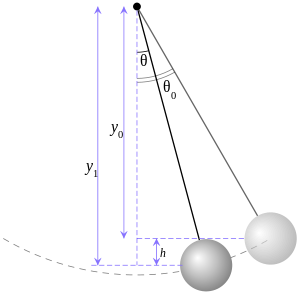
\includegraphics[width=6.0cm]{pendulo.png}
      \caption{Péndulo simple \cite{Img1}.}
    \end{center}
\end{wrapfigure}
Como nos dice \cite{Wik} "Las matemáticas de un péndulo son, en general, muy complicadas. Asumir simplificaciones, en el caso de un péndulo simple. nos permite resolver las ecuaciones analíticamente para oscilaciones de ángulos pequeños."
Por esto mismo es que se toma el modelo del péndulo simple, es decir, utilizamos una seria de idealizaciones que nos permiten un estudio del mismo más sencillo que si no las tomáramos de esta forma; las condiciones que se asumen son:\\

\begin{itemize}
\item El cordón al cual se sujeta el peso posee una masa despreciable, además de ser rígido.
\item El peso se considera una masa puntual.
\end{itemize}
\pagebreak

\begin{itemize}
\item El movimiento solo ocurre en dos dimensiones, por lo que el peso no traza una elipse, si no un arco.
\item El péndulo no pierde energía ya que no se considera la fricción con el aire.
\item El campo gravitacional es uniforme.
\item El soporte no se mueve.
\end{itemize}

De igual modo, sabemos que se toma este modelo se toma únicamente para movimientos en ángulos pequeños, ya que de ser diferente las ecuaciones que describen el movimiento del péndulo se complican.

\subsection*{\textcolor{NavyBlue}{Aproximaciones para ángulos pequeños.}}
A pesar de no resultar fácil resolver la ecuación diferencial que describe el movimiento de un péndulo, si a este se le restringe su ángulo de oscilación a menos de 1 radian, la ecuación puede resolverse de una forma sencilla.
\begin{eqnarray*}
\sin \theta \approx \theta \\
\frac{d^2 \theta}{dt^2} + \frac{g}{l}\theta = 0
\end{eqnarray*}

Tomando como condiciones iniciales $\theta (0) = \theta_0$ y $d\theta l dt(0) = 0$, la solución resulta en:
\begin{eqnarray*}
\theta(t) = \theta_0 \cos \left( \sqrt{\frac{g}{l}t} \right)  \qquad \theta_0 \ll 1 
\end{eqnarray*}

\subsection*{\textcolor{NavyBlue}{Amplitudes arbitrarias.}}
Cuando se trabaja con amplitudes más grandes, es posible, por medio de un programa computacional, calcular el periodo exacto invirtiendo la ecuación de la velocidad angular obtenida por medio de la energía:

\begin{eqnarray*}
\textcolor{Red}{\frac{dt}{d \theta} = \sqrt{\frac{l}{2g}} \frac{1}{\sqrt{\cos\theta -  \cos\theta_0}}}
\end{eqnarray*}

y después integrando sobre un ciclo completo
\begin{eqnarray*}
T = t(\theta_0 \to 0 \to -\theta_0 \to 0 \to \theta_0)
\end{eqnarray*}

o dos veces un medio ciclo
\begin{eqnarray*}
T=2t(\theta_0 \to 0 \to -\theta_0)
\end{eqnarray*}

o cuatro veces un cuarto de ciclo
\begin{eqnarray*}
T=4t(\theta_0 \to 0)
\end{eqnarray*}

lo cual nos lleva a
\begin{eqnarray*}
T=4 \sqrt{\frac{l}{2g}}\int\limits_0^{\theta_0} \frac{1}{\sqrt{\cos\theta - \cos\theta_0}} d\theta
\end{eqnarray*}


\pagebreak
\section*{\textcolor{LimeGreen}{Problema.}}
La actividad a realizar esta vez, consiste simplemente en comprender a grandes rasgos la forma en que trabaja un código que se nos proporcionó que realiza la simulación de un modelo de péndulo simple y en observar si este arroja datos consistentes :

\begin{verbatim}
#theta'(t) = omega(t)
#omega'(t) = -b*omega(t) - c*sin(theta(t))

def pend(y, t, b, c):
     theta, omega = y
     dydt = [omega, -b*omega - c*np.sin(theta)]
     return dydt

b = 0.0 #fricción
g = 9.8 #gravedad
l = 5 #longitud de la cuerda
c = g/l

y0 = [np.pi/2, 0.02] #ángulo inical, velocidad angular

t = np.linspace(0, 20, 500) #rango de tiempo

from scipy.integrate import odeint
sol = odeint(pend, y0, t, args=(b, c))

import matplotlib.pyplot as plt
plt.plot(t, sol[:, 0], 'b', label='theta(t)') 
#theta = posición
plt.plot(t, sol[:, 1], 'g', label='omega(t)') 
#omega = velocidad angular
plt.legend(loc='best')
plt.xlabel('t')
plt.grid()
plt.show()
\end{verbatim}

Podemos observar que el código define de una manera simple la segunda coordenada de $dydt$ utilizando la forma homogénea de la ecuación diferencial del péndulo, para lo cual se define $b$ y $c$. De igual forma resulta sencillo comprender todas aquellas definiciones que se dan para las diferentes variables utilizadas en el código, hasta que llegamos al punto de definir $sol$ para lo cual utilizamos la herramienta $odeint$ importada desde $scipy.integrate$; la cual utilizamos para integrar un sistema de ecuaciones diferenciales simples utilizando Isoda desde la librería odepack de Fortran.\\
Para realizar esta operación es necesario identificar algunos parámetros en orden:
\begin{itemize}
\item y0.- correspondiente a las condiciones iniciales del problema.
\item t.- una secuencia de puntos para los cuales resolver la ecuación.
\item args.- argumentos extras para realizar la función.
\end{itemize}
Finalmente de grafica cada una de las columnas del arreglo que nos regresa la función $odeint$ y de esta forma obtenemos la gráfica tanto de la posición como de la velocidad angular del péndulo para cada punto en el rango de tiempo que especifiquemos.



\pagebreak

\section*{\textcolor{RoyalBlue}{Resultados}}
Utilizando el código que se nos proporcionó podemos realizar pruebas para distintos escenarios modificando todo aquel factor que deseemos, ya sea el coeficiente de fricción, la gravedad, la longitud de la cuerda del péndulo, su ángulo inicial o la velocidad que este tendrá inicialmente.\\
Modelaremos cuatro diferentes escenarios, cada uno con distintos factores y observaremos si sus gráficas corresponden al comportamiento que este debe de tener.\\
\begin{itemize}
\item Coeficiente de fricción = 0
\item Aceleración por la gravedad = 9.8
\item Longitud de la cuerda = 2
\item Posición inicial = $\frac{\pi}{2}$
\item Velocidad inicial = 0.08
\end{itemize}

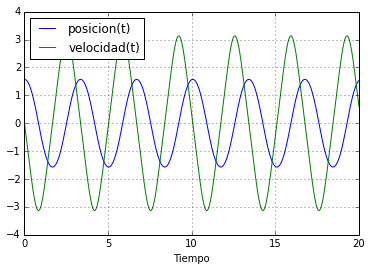
\includegraphics{5a.png}

\begin{itemize}
\item Coeficiente de fricción = 0
\item Aceleración por la gravedad = 9.8
\item Longitud de la cuerda = 2
\item Posición inicial = $\frac{\pi}{2}$
\item Velocidad inicial = 0.0
\end{itemize}

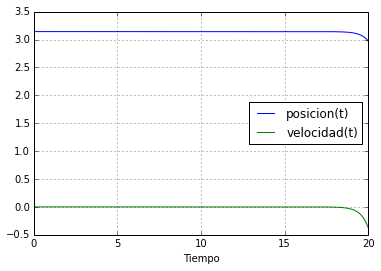
\includegraphics{5b.png}
\pagebreak
\begin{itemize}
\item Coeficiente de fricción = 0
\item Aceleración por la gravedad = 9.8
\item Longitud de la cuerda = 5
\item Posición inicial = $\frac{3\pi}{4}$
\item Velocidad inicial = 0.5
\end{itemize}

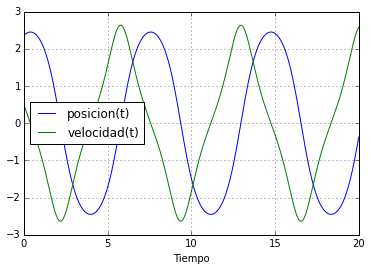
\includegraphics{5c.png}
\pagebreak
\begin{itemize}
\item Coeficiente de fricción = 0.4
\item Aceleración por la gravedad = 9.8
\item Longitud de la cuerda = 4.5
\item Posición inicial = $\frac{\pi}{3}$
\item Velocidad inicial = 0.9
\end{itemize}
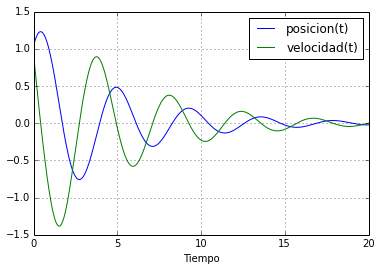
\includegraphics{5d.png}
\pagebreak
\begin{thebibliography}{X}
 \bibitem{1} \textsc{Wikipedia, The free encyclopedia; "Pendulum"; 2016}
 \bibitem{Wik} \textsc{Wikipedia, The free encyclopedia; "Pendulum (mathematics)"; 2016}
 \bibitem{3} \textsc{Wikipedia, The free encyclopedia; "Numerical methods for orfinary differencial equations"; 2016}
 \bibitem{4} \textsc{Wikipedia, The free encyclopedia; "Euler method"; 2016}
 \bibitem{Img1} \textsc{By Krishnavedala; via Wikimedia Commons;"Pendulum (mathematics)"}
 \bibitem{5} \textsc{scipy.integrate.odeint de Python}
\end{thebibliography}
\end{document}